\documentclass[12pt, toc = bibliography, english]{scrreprt} %display bibliography in table of contents
\usepackage[utf8]{inputenc} %input encoding
\usepackage[T1]{fontenc} %font encoding
\usepackage{lmodern} %font
\usepackage{babel}
\usepackage{pdfpages} %allow import of pdf
\usepackage[hidelinks]{hyperref} %do not display links underlined and in color
\usepackage{bookmark} % for hyperref
\usepackage[backend=biber, citestyle=ieee, sorting=none]{biblatex} %bibliography
\usepackage{csquotes} %german quote style
\usepackage{acro} %acronyms
\usepackage[a4paper,left=3cm, right = 2cm]{geometry} %size of document
\usepackage{setspace}
\usepackage{parskip} % do not make indentations at paragraphs
\usepackage{float} %allow [H] for images to stay where you want them
\usepackage{xcolor}
\usepackage{fancyhdr}
\usepackage{xurl} %avoid overful hbox by breaking urls everywhere
\usepackage{listings} % Für Code-Listings
\usepackage{adjustbox}
\usepackage{pgfplots}
\usepackage{tikz}
\usepackage{pgfplotstable}

\definecolor{treeBlue}{HTML}{00a8f3}
\definecolor{treeGreen}{HTML}{0ed145}
\definecolor{tableGreen}{HTML}{5ea06e}
\definecolor{tableBlue}{HTML}{187eca}
\definecolor{excelOrange}{HTML}{ffcc99}
\definecolor{excelGreen}{HTML}{00b050}
% Farbdefinitionen
\definecolor{codegray}{gray}{0.90} % Hellgrauer Hintergrund
\definecolor{codeblack}{gray}{0} % Hellgrauer Hintergrund

\definecolor{codegreen}{rgb}{0,0.6,0}
\definecolor{codeblue}{rgb}{0,0,1}
\definecolor{codered}{rgb}{0.6,0,0}
\definecolor{codepurple}{rgb}{0.58,0,0.82}
\definecolor{commentcolor}{rgb}{0.5,0.5,0.5} % Kommentarfarbe

\renewcommand{\rmdefault}{lmr} % Arial
\renewcommand{\sfdefault}{lmr} % Arial
\RedeclareSectionCommand[
 beforeskip=0cm % reduce margins at chapters
]{chapter}
\fancyhead[C]{}
\fancyhead[R]{}        
\pagestyle{fancy} %fancy header: only display chapter
\fancyhead[L] {
    \leftmark{}
}                
\linespread{1.25} %entspricht 1,5 in word
% \counterwithout{figure}{chapter} %Abb.1 not Abb.[chapter].1

% \renewcommand{\chaptername}{\MakeUppercase{\@chapapp}}
% \renewcommand{\addcontentsline}[3]{\protected\addcontentsline{#1}{#2}{\protect\MakeUppercase{#3}}}

\lstdefinestyle{mystyle}{
   backgroundcolor=\color{codegray},  % Hintergrundfarbe
   commentstyle=\color{commentcolor},
   keywordstyle=\color{codeblue},
   numberstyle=\tiny\color{codeblack},
   stringstyle=\color{codepurple},
   basicstyle=\ttfamily\footnotesize,
   breakatwhitespace=false,
   breaklines=true,
   captionpos=b,
   keepspaces=true,
   numbers=left,
   numbersep=5pt,
   showspaces=false,
   showstringspaces=false,
   showtabs=false,
   tabsize=2,
%    language=C,
   postbreak=\mbox{\textcolor{red}{$\hookrightarrow$}\space}
}

\lstset{style=mystyle}



\DeclareAcronym{msrp}{
	short = MSRP,
	long = manufacturer's suggested retail price
}

\DeclareAcronym{csv}{
	short = CSV,
	long = Comma-separated values
}

\DeclareAcronym{vw}{
	short = VW,
	long = Volkswagen
}

\DeclareAcronym{excel}{
	short = Excel,
	long = Microsoft Excel
}

\DeclareAcronym{mpg}{
	short = MPG,
	long = miles per gallon
}

\DeclareAcronym{vscode}{
	short = VS Code,
	long = Visual Studio Code
}

\DeclareAcronym{mse}{
	short = MSE,
	long = Mean-squared error
}

\DeclareAcronym{r2}{
	short = ${r}^2$,
	long = coefficient of determination
} 
\addbibresource{sources.bib}

\begin{document}
\title{Business analytics \\ Analysis of car advertisement data}
\author{Alina Ivanova, Moritz Hangen, Simon Gosch}
\date{2024/03/24}
\maketitle

\tableofcontents
\listoffigures
\addcontentsline{toc}{chapter}{\listfigurename} %Abbildungsverzeichnis in table of content
\listoftables
\addcontentsline{toc}{chapter}{\listtablename} %Abbildungsverzeichnis in table of content

\chapter{Introduction}
As of 2023, a compound annual growth rate of 10\% was forecast for the world used car market between 2024 and 2029.
There are a lot of factors that may cause such a significant growth, including shorter vehicle ownership times, changes in preferences for cars, and increasing flexibility of supply \autocite{UsedCarMarket}.
The market growth and upward trend in the demand for cost-effective used cars \autocite{EuropeUsedCar} raise the necessity of proper price calculations for resale cars, since it affects both car dealers and clients.
It should estimate the accurate value of the vehicle based on its condition. Moreover, the initial set price of the car is significant for the final revenue received from the dealership.

This paper addresses the business problem of determining competitive prices for used cars to be advertised.
For the accuracy of the analysis, only one car model was chosen: the \ac{vw} Golf, as it is one of the most popular cars on used car market in such countries as Germany, Belgium, Italy and others \autocite{misselhornDevelopmentUsedCar2024}.
The following research questions were posed: 
\newline
 1) What factors influence \ac{vw} Golf's price the most? \newline
 2) What is the price the \ac{vw} Golf should be advertised for?\newline
To answer the questions, correlation and linear regression were calculated, and the model has been created. The programs used for the analysis are \ac{excel} and Orange.
The research was based on a large-scale dataset for automotive applications, which contained various data for 0.25 million used cars in the United Kingdom. For research purposes, only a part about used car advertisements was used.


\chapter{Theoretical background}
\section{Correlation}

In simple terms, a correlation coefficient shows if two variables are dependent. The correlation coefficient varies from -1 to 1. The closer it is to extreme values, the stronger the variables are related. If the correlation coefficient is positive, that means that variables move in the same direction; for instance, when demand is growing, prices are increasing, and if demand decreases, prices go down as well. A negative correlation shows the opposite relationship. For example, when supply rises, prices drop, and vice versa. The correlation of 0 indicates that variables are independent \autocite{DaCostaLewis2005}.
There are various types of correlations. Pearson and Spearman are two of the most common correlations. It is a measure of strength and direction of linear relationship in data with normally distributed values. Alternatively, Spearman correlation is used to analyze data that is non-normally distributed
\autocite{schoberCorrelationCoefficientsAppropriate2018}.

\section{Linear regression}

Linear regression is a statistical tool that helps to predict the value of a targeted dependent variable based on other attributes. An important measure in linear regression analysis is the \ac{r2}. It represents the percentage of cases where the change in an independent variable can be explained by the change in a dependent one. The \ac{r2} varies between 0 and 1. The closer it is to 1, the stronger the linear relationship between variables
\autocite{kumariLinearRegressionAnalysis2018}.
\ac{mse} is another vital measure to consider. It displays the difference between predicted and actual values in a regression model, as well as how much predictions change across different data sets. The smaller the MSE, the more accurate and reliable the predicted values are
\autocite{Schluchter2005}.
\section{Data}
We explored a large-scale dataset for automotive applications which originally consisted of 7 files:
\begin{itemize}
    \item "Ad\_table": Contained information about more than 0.25 million used car advertisements
    \item "Ad\_table (extra)": “Ad\_table” information with additional car characteristics
    \item "Basic\_table": information about car attributes
    \item "Image\_table": car images attributes
    \item “Price\_table”: entry-level new car prices for 1998-2021
    \item “Sales\_table”: ten years car sales data in UK
    \item “Trim\_table”: trim attributes including the engine type and engine size
\end{itemize}
“Ad\_table (extra)” was used for the research purposes. It shows data about used car advertisements for more than 80 different car brands in 2016-2018. The dataset contains information about cars' maker and models, month and year of the advertisement, cars' year of registration, body type, color, ran miles, engine size in liters, and engine power in horsepower, gearbox (automatic, manual, semi-automatic), fuel type (diesel, electric, hybrid petrol/electric plug in, petrol), the price and annual tax in pounds, wheelbase in millimeters, cars dimensions: height, width, and length in millimeters; average miles per gallon; top speed in miles per hour; the number of seats and doors. In addition, there are attributes for model ID and advertisement ID
\autocite{huangDVMCARLargescaleAutomotive2022}.

\chapter{Analysis}
\section{Analysis method}
The goal is to make a data driven decision on how much a \ac{vw} Golf arriving at the dealership should be advertised for,
based on the car's specifications, assuming there is some kind of dependence.
To check whether this dependence exists, the correlations between the specifications and the price are evaluated.
After that, to get a model that predicts the price based on the other attributes, linear regression is used.
Its simplicity when it comes to understanding and calculating the model, as well as interpreting the results, make it well-suited
for this use case.    

\section{Data processing}
\subsection{Preprocessing in Excel}
First step of preprocessing the data is the reduction to only data points with the value \enquote{\ac{vw} Golf} for the car model attribute. Therefore, the \ac{csv} file containing the raw data is
imported into \ac{excel}, and a filter to the car model column is applied. As some cells are blank for certain attributes, another filter removing the affected rows is set for every column. 

\subsection{Preparations for Orange}
After the previous steps, the data set is still not ready to be processed in Orange. The problem is that certain cells not only contain the actual numeric value but also the 
unit. For example the column of the car's average \ac{mpg} always has the text \enquote{mpg} after the value, causing Orange to not recognize it as 
numeric value. To fix this issue, the \ac{csv} file is opened in a text editor, and its \enquote{Find and replace} functionality is used to replace the unit with blank text.
This is working as the texts,
which have to be removed, only appear in two other places, where they are manually added back. So both the \enquote{mpg} from the average \ac{mpg} column and the \enquote{L}
from the engine size column were removed like this.

\subsection{Processing in Orange}
To understand how each attribute affects the car's price, the correlations are calculated using the Pearson correlation coefficient. 
\begin{figure}[h]
    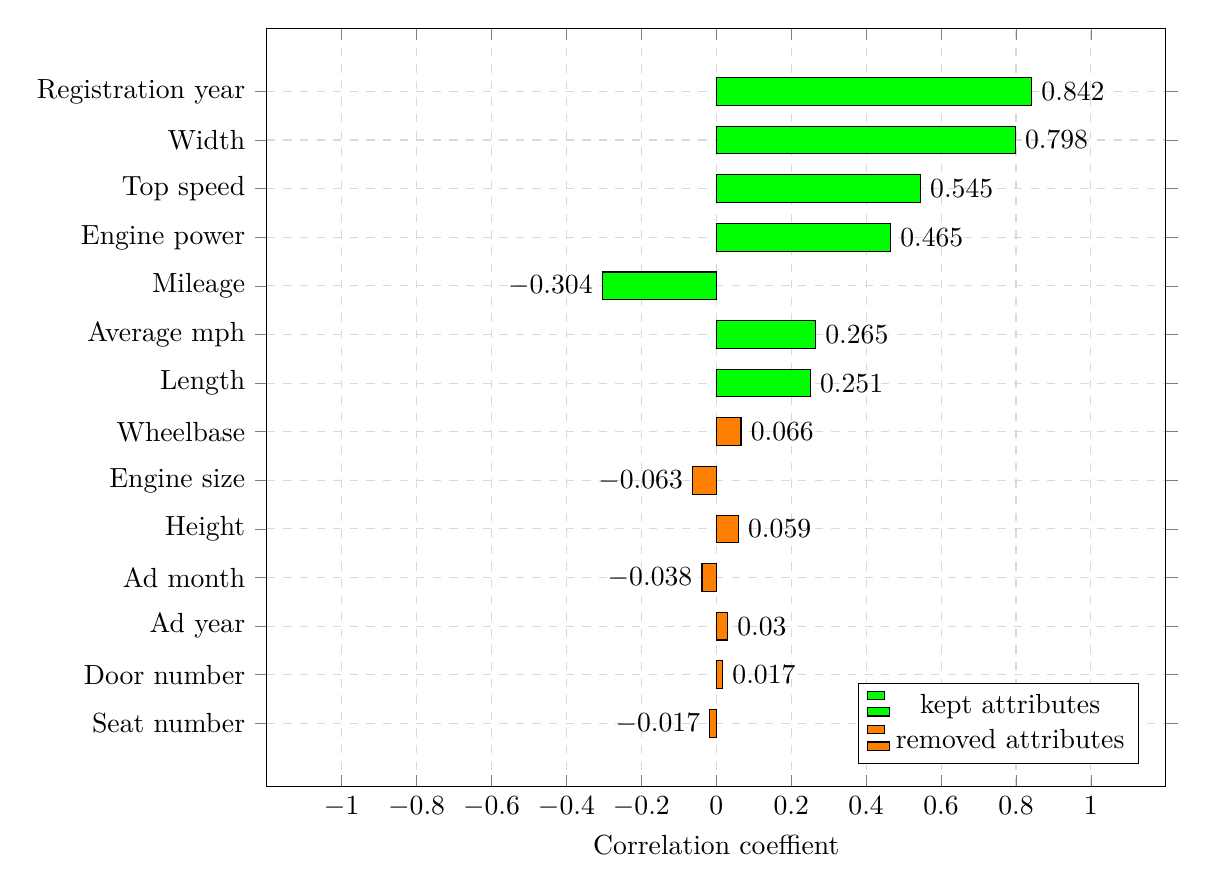
\begin{tikzpicture}
        \begin{axis}[
            xbar,
            xmin=-1.2,
            xmax=1.2,
            xtick={-1,-0.8,-0.6, -0.4, -0.2, 0, 0.2, 0.4, 0.6, 0.8, 1},
            legend pos=south east,
            grid=major, grid style={dashed,gray!30},
            width=13cm,
            xlabel={Correlation coeffient},
            symbolic y coords={Seat number,Door number,Ad year,Ad month,Height,Engine size,Wheelbase,Length,Average mph,Mileage,Engine power,Top speed,Width,Registration year},
            ytick={Seat number,Door number,Ad year,Ad month,Height,Engine size,Wheelbase,Length,Average mph,Mileage,Engine power,Top speed,Width,Registration year},
            nodes near coords,
            nodes near coords align={horizontal},
            every node near coord/.style={/pgf/number format/fixed, /pgf/number format/precision=3},
            /pgf/bar shift={0pt},
            ]
            \addplot [fill=green] coordinates {
                (0.251,Length)
                (0.265,Average mph)
                (-0.304,Mileage)
                (0.465,Engine power)
                (0.545,Top speed)
                (0.798,Width)
                (0.842,Registration year)
                };
            \addplot [fill=orange] coordinates {
                (-0.017,Seat number)
                (0.017,Door number)
                (0.03,Ad year)
                (-0.038,Ad month)
                (0.059,Height)
                (-0.063,Engine size)
                (0.066,Wheelbase)
                };
            \legend{kept attributes, removed attributes}
        \end{axis}
    \end{tikzpicture}
    \caption{Correlation with the price attribute}
    \label{fig:correlationdiagram}
\end{figure}
\par
\autoref{fig:correlationdiagram} shows a horizontal bar chart visualizing the correlation coefficient for each attribute.
As a bar chart lists the different values of the coefficients side by side in an easy-to-read way, it is perfect for the 
given purpose of focusing on comparison between the attributes. 
The horizontal layout allows good readability for the long labels and is more suitable for placing the actual values next to the
bars, as there are no space limitations along the y-axis. 
\par
Having the results of the correlation analysis allows to answer the first research question: \enquote{What factors influence Volkswagen Golf's price the most?}.
\autoref{fig:correlationdiagram} provides the answer, as the attributes are listed from highest to lowest influence on the price. Those highlighted in green
have a significant impact, while the rest do not. Therefore, those highlighted in orange are not taken into account for the further data analysis.

\par
In the next step, not only the attributes with low correlation but also the non-numeric ones are removed. This is the case as they can't be used in the calculation
of the linear regression model without further preprocessing. These additional preprocessing steps are not performed as the resulting linear regression
model is already very good. 
Additionally, the price is set as target value for the linear regression calculation.

\par
As a final step, the data set is split into training and test data, and the linear regression model is calculated based on the
training data. Insights about the training split, as well as quality and specifications of the model, are discussed in the next section of the report. 

\section{Linear regression model}
\subsection{Specifications}
For the calculation of the linear regression model, a training split of 60\% training and 40\% test data is used.
When testing the model, the results are very satisfactory with a \ac{mse} of 3750250.922 and \ac{r2} of 0.912.
Especially, the \ac{r2} being very close to 1 indicates a high linear relationship between the model and the target attribute,
which means that the model predicts the price accurately.

\subsection{Visualization}
The reason for visualizing the linear regression model is that it is always easier to analyze and interpret visual 
results rather than only working with numeric values.
Used for that matter is a scatter plot, shown in \autoref{fig:linearregressiondiagram}. 
\begin{figure}[h]
    \begin{tikzpicture}
        \begin{axis}[
            clip mode=individual,
            legend pos=south east,
            xmin=400,
            xmax=20000,
            ymin=400,
            ymax=20000,
            xlabel={Actual price \lbrack\pounds\rbrack},
            ylabel={Model's calculated price \lbrack\pounds\rbrack},
            xtick={2000, 6000, 10000, 14000, 18000},
            ytick={2000, 6000, 10000, 14000, 18000},
            width=13cm,
            scaled ticks=false,
            tick label style={/pgf/number format/fixed},
            y label style={yshift=1.2em}
            ]
        \addplot [mark=none,color=blue,style=very thick]
          table [y={create col/linear regression={y=model_price}}, col sep=comma] {./other/Linear_regression.csv};
          \addlegendentry{Regression line}  
          \addplot [mark=*,color=red,only marks, fill opacity = 0.35, draw opacity = 0]
          table [x=actual_price, y=model_price, col sep=comma] {./other/Linear_regression.csv};
                 
        \end{axis}
      \end{tikzpicture}
    \caption{Plotted Linear Regression Model}
    \label{fig:linearregressiondiagram}
\end{figure}
\par
Scatter plots are optimal to show the relationship between two variables, in this case, the actual price from the test data 
and the price predicted by the linear regression model. The closer the data points are to the regression line, the 
better the model performs. By knowing this, it is easy to analyze the quality of the model, even without any prior knowledge.
So, when looking at \autoref{fig:linearregressiondiagram}, one can see that the data points portray the regression line 
quite precisely. This reinforces the prior statement that the linear regression model is very good.


\chapter{Findings and discussion}
\section{Model usage}
Given the regression model, it can be applied to example data to examine its behavior.
\subsection{Assessing expectations}
Intuitive assumptions draw you to the conclusion, that the vehicle's mileage has an inverse relationship to the predicted advertisement price.
\begin{table}[H]
    \begin{adjustbox}{width={\textwidth}}
        \begin{tabular}{|l|l|l|l|l|l|l|l|}
            \hline
            Registration year & \textbf{Mileage} & Horsepower & Width (mm) & Length (mm) & Average mpg & Top speed (mph) & \textbf{Predicted price} \\ \hline
            2017              & \textbf{60000}   & 135        & 2027       & 4284        & 49          & 116             & \textbf{16157}           \\\hline
            2017              & \textbf{130000}  & 135        & 2027       & 4284        & 49          & 116             & \textbf{13828}           \\\hline
        \end{tabular}
    \end{adjustbox}
    \caption{Influence of mileage on recently registered cars}
    \label{mileage_data_new_car}
\end{table}
As it can be observed in \autoref{mileage_data_new_car}, a higher mileage in fact reduces the predicted price.
However, for an over 2-fold increase in miles, the depreciation is with 14.4 \% not as high as expected.
\par
While comparing two otherwise identical cars, it should be noted that the other values still contribute significantly to the
result.
\newline
In particular the registration year, which, as shown before, strongly correlates with the target variable has an effect on the limited
influence of the mileage here.
Given the dataset's sampling of data up to 2017, both of the \ac{vw} Golfs in\autoref{mileage_data_new_car} have been first registered only one year ago, so the base price is measurably higher.
If you apply the same example to cars registered in 2010, which therefore have been running for seven years, the influence of the mileage grows.
\begin{table}[H]
    \begin{adjustbox}{width={\textwidth}}
        \begin{tabular}{|l|l|l|l|l|l|l|l|}
            \hline
            \textbf{Registration year} & \textbf{Mileage} & Horsepower & Width (mm) & Length (mm) & Average mpg & Top speed (mph) & \textbf{Predicted price} \\ \hline
            \textbf{2010}              & \textbf{60000}   & 135        & 2027       & 4284        & 49          & 116             & \textbf{11122}           \\\hline
            \textbf{2010}              & \textbf{130000}  & 135        & 2027       & 4284        & 49          & 116             & \textbf{8793}           \\\hline
        \end{tabular}
    \end{adjustbox}
    \caption{Influence of mileage on older cars}
    \label{mileage_data_old_car}
\end{table}
As shown in \autoref{mileage_data_old_car}, the gap between the two otherwise identical vehicles has widened to 20.9 \%, a sharp increase by 45.2 \%.


\subsection{Usage of example data}
\begin{table}[H]
    \begin{adjustbox}{width={\textwidth}}
        \begin{tabular}{|l|l|l|l|l|l|l|l|}
            \hline
            Registration year & Mileage & Horsepower & Width (mm) & Length (mm) & Average mpg & Top speed (mph) & \textbf{Predicted price (£)} \\\hline
            2014              & 180000  & 110        & 1799       & 4204        & 45          & 110             & \textbf{5601}                \\\hline
            2016              & 150000  & 120        & 2027       & 4255        & 48          & 112             & \textbf{12130}               \\\hline
            2018              & 80000   & 130        & 2027       & 4255        & 50          & 115             & \textbf{16136}               \\\hline
            2015              & 190000  & 115        & 1799       & 4204        & 44          & 108             & \textbf{5819}                \\ \hline
        \end{tabular}
    \end{adjustbox}
    \caption{Assessing model for business use cases}
    \label{predicted_price_realworld_data}
\end{table}
\section{Findings}
\subsection{In line with presumptions}
\subsubsection{Mileage $\leftrightarrow$ Price}
\subsubsection{Engine size $\leftrightarrow$ Price}

\subsection{Outliers}
\subsubsection{Engine size $\leftrightarrow$ Price}
\subsubsection{Width $\leftrightarrow$ Price}
\subsubsection{Year $\leftrightarrow$ Price}
TODO include example of higher influence of mileage the older the car is

\chapter{Conclusion}
\section{Summary}
\section{Further questions}


\printbibliography
\end{document}
